\documentclass[sigconf]{acmart}
% \documentclass{...}
%\documentclass[11pt, letterpaper]{article}
\usepackage[margin=1in]{geometry}

% \documentclass[11pt, letterpaper]{article}
% 
% % ----- margins -----
% 
% \topmargin -1.5cm         % read Lamport p.163
% \oddsidemargin -0.04cm    % read Lamport p.163
% \evensidemargin -0.04cm   % same as oddsidemargin but for left-hand pages
% 
% % ----- texts -----
% 
% \textwidth 16.59cm
% \textheight 21.94cm
% 
% % ----- indendts and spacing -----
% 
% \parskip 0pt            	% spacing between paragraphs
% %\renewcommand{\baselinestretch}{1.5}	% uncomment for 1.5 spacing
% 
% \parindent 7mm		      % leading space for paragraphs between lines
% 
% % ----- page # -----
% 
% %\pagestyle{empty}         % uncomment if don't want page numbers





%=== use the these packages if they are not already in use ===
%\usepackage{amsfonts}
%\usepackage{amsmath}
%\usepackage{amssymb}
\usepackage{amsthm}
\usepackage{bbm} 
%\usepackage{cite}
\usepackage{color}
%\usepackage{euscript}
\usepackage{graphicx}
\usepackage{mathrsfs} 
%\usepackage{microtype}
% \usepackage[normalem]{ulem}
% \usepackage{wrapfig}
%=============================================================

%===== control =====
\allowdisplaybreaks

%===== fonts =====
\def\ttt{\texttt}
\def\tsc{\textsc}

%===== spacing =====

\def\extraspacing{\vspace{3mm} \noindent}
\def\figcapup{\vspace{-1mm}}
\def\figcapdown{\vspace{-0mm}}
\def\hgap{\textrm{\hspace{1mm}}}
\def\thmvgap{\vspace{0mm}}
\def\vgap{\vspace{1mm}}


%===== tabbing =====

\def\tab{\hspace{3mm}}
\def\tabpos{\hspace{4mm} \= \hspace{4mm} \= \hspace{4mm} \= \hspace{4mm} \= \hspace{4mm} \= \hspace{4mm} \= \hspace{4mm} \= \hspace{4mm} \= \hspace{4mm} \= \hspace{4mm} \= \hspace{4mm} \= \hspace{4mm} \= \hspace{4mm} \= \hspace{4mm} %\= 
%\= \hspace{4mm} \= \hspace{4mm} \= \hspace{4mm} \= \hspace{4mm} \= \hspace{4mm} \= \hspace{4mm}
\kill}
\newcommand{\mytab}[1]{\begin{tabbing}\tabpos #1\end{tabbing}}

%===== blocks =====

%%%%%%%%%%%%%%%%%%%%%%%%%%%%%%%%
% THEOREMS
%%%%%%%%%%%%%%%%%%%%%%%%%%%%%%%%
% \theoremstyle{plain}
% \newtheorem{theorem}{Theorem}[section]
% \newtheorem{proposition}[theorem]{Proposition}
% \newtheorem{lemma}[theorem]{Lemma}
% \newtheorem{corollary}[theorem]{Corollary}
% \theoremstyle{definition}
% \newtheorem{definition}[theorem]{Definition}
% \newtheorem{assumption}[theorem]{Assumption}
% \theoremstyle{remark}
% \newtheorem{remark}[theorem]{Remark}

% \newtheorem{theorem}{Theorem}
% \newtheorem{lemma}[theorem]{Lemma}
% \newtheorem{corollary}[theorem]{Corollary}
% \newtheorem{proposition}{Proposition}
% \newtheorem{definition}{Definition}
% \newtheorem{problem}{Problem}

\newcommand{\boxminipg}[2]{\begin{center}\fbox{\begin{minipage}{#1}#2\end{minipage}}\end{center}}
\newcommand{\minipg}[2]{\begin{center}\begin{minipage}{#1}#2\end{minipage}\end{center}}
\newcommand{\myitems}[1]{\begin{itemize} #1 \end{itemize}}
\newcommand{\myenums}[1]{\begin{enumerate} #1 \end{enumerate}}
\newcommand{\myfig}[1]{\begin{figure}\centering #1\end{figure}}
\newcommand{\myfigg}[2]{\begin{figure}\centering #1 \figcapup \caption{#2} \figcapdown \end{figure}}
\newcommand{\myfigstar}[2]{\begin{figure*}\centering #1 \figcapup \caption{#2} \figcapdown \end{figure*}}

%===== math macros =====

\newcommand{\bm}[1]{\textrm{\boldmath${#1}$}}
\newcommand{\mb}[1]{\mathbf{#1}}
% \newcommand{\smat}[2]{\left[\begin{tabular}{#1}#2\end{tabular}\right]}
% \newcommand{\bmat}[2]{\left|\begin{tabular}{#1}#2\end{tabular}\right|}
\newcommand{\bmat}[1]{\begin{bmatrix}#1\end{bmatrix}}
\newcommand{\vmat}[1]{\begin{vmatrix}#1\end{vmatrix}}
\newcommand{\myeqn}[1]{\begin{eqnarray}#1\end{eqnarray}}
\newcommand{\myset}[1]{\{#1\}}
\newcommand{\set}[1]{\{#1\}}

\newcommand{\explain}[1]{(\textrm{#1})}
%\newcommand{\bracket}[1]{\left(#1\right)}
%\newcommand{\dbar}[1]{\Vert#1\Vert}
%\newcommand{\one}[1]{\mathbbm{1}\{#1\}}

%\def\bm{\boldmath}
%\def\defeq{\stackrel{\textrm{\tiny{def}}}{=}}
\def\mit{\mathit}
\def\defeq{:=}
\def\eps{\epsilon}
\def\fr{\frac}
\def\-{\mbox{-}}
\def\ol{\overline}
\def\real{\mathbb{R}}
\def\intdom{\mathbb{N}}

\def\tO{\tilde{O}}
\def\tOmega{\tilde{\Omega}}

\def\lc{\left \lceil}
\def\lf{\left \lfloor}
\def\rc{\right \rceil}
\def\rf{\right \rfloor}
\newcommand{\ceil}[1]{\lceil #1 \rceil}
\newcommand{\floor}[1]{\lfloor #1 \rfloor}

\def\nn{\nonumber}

\def\Pr{\mathbf{Pr}}
%\def\expt{\mathbf{E}}
\def\var{\mathbf{Var}}

\def\dcl{\{\!\!\{}
\def\dcr{\}\!\!\}}
\def\bigdcl{\Big\{\!\!\Big\{}
\def\bigdcr{\Big\}\!\!\Big\}}
\def\bigmid{\textrm{ $\Big|$ }}


\DeclareMathOperator*{\argmin}{arg\,min}
\DeclareMathOperator*{\argmax}{arg\,max}
\DeclareMathOperator*{\polylog}{polylog}
\DeclareMathOperator*{\poly}{poly}
\DeclareMathOperator*\expt{\mathbf{E}}
%\DeclareMathOperator*\Pr{\mathbf{Pr}}

%===== misc =====

\def\done{\qed \vspace{2mm}}	% end of proof
\def\tbc{\hspace*{\fill} $\textrm{{\em (to be continued)}}\blacktriangle$ \vspace{2mm}}
%\def\done{\hspace*{\fill} $\Box$}	% end of proof
\allowdisplaybreaks
%===== coloring =====

\newcommand{\red}[1]{\textcolor{red}{#1}}
\newcommand{\blue}[1]{\textcolor{blue}{\bf #1}}
\newcommand{\purple}[1]{\textcolor{purple}{\bf #1}}
\newcommand{\todo}[1]{\textcolor{red}{\bf [TO DO: #1]}}


%=================================
%Yufei's stuff
%\usepackage{amsmath}
\usepackage{balance}
%\usepackage{times}
\usepackage{microtype}

\def\vgap{\vspace{1mm}}
\def\extraspacing{\vspace{2mm} \noindent}
\def\figcapup{\vspace{-0mm}}
\def\figcapdown{\vspace{-0mm}}

\def\A{\mathcal{A}}
\def\B{\mathcal{B}}
\def\C{\mathcal{C}}
\def\E{\mathcal{E}}
\def\G{\mathcal{G}}
\def\I{\mathcal{I}}
\def\J{\mathcal{J}}
\def\II{\mathscr{I}}
\def\L{\mathcal{L}}
\def\P{\mathcal{P}}
\def\Q{\mathcal{Q}}
\def\R{\mathcal{R}}
\def\T{\mathcal{T}}
\def\U{\mathcal{U}}
\def\V{\mathcal{V}}
\def\X{\mathcal{X}}
\def\XX{\mathscr{X}}
\def\Y{\mathcal{Y}}
\def\YY{\mathscr{Y}}
\def\Z{\mathcal{Z}}

\def\out{\mathrm{OUT}}

\allowdisplaybreaks
%=================================

%====== from acm ======
\acmDOI{}
\acmISBN{}

\acmConference[]{...}{...}{...}
\acmYear{...}
\copyrightyear{}
\acmArticle{}
\acmPrice{}
%======================



\begin{document}
%\begin{sloppy}
    
\title{Optimal (Multiway) Spatial Joins}

% \author{}
% \affiliation{
% 	\institution{Chinese University of Hong Kong}
% 	\city{Hong Kong}
% 	\country{China}}	

\author{}


\begin{abstract}
    In a {\em spatial join}, we are given a constant number $k \geq 2$ of sets containing axis-parallel rectangles in a 2D space, denoted as $R_1, R_2, ..., R_k$. The objective is to report all $k$-tuples $(r_1, r_2, ..., r_k) \in R_1 \times R_2 \times ... \times R_k$ where the rectangles $r_1, r_2, ..., r_k$ have a non-empty intersection, i.e., $r_1 \cap r_2 \cap ... \cap r_k \neq \emptyset$. This problem holds significant importance in spatial databases and has been extensively studied for over two decades. We explain how to settle the problem in $O(n \log n + \out)$ time using $O(n + \out)$ space --- regardless of the constant $k$ --- where $n = \sum_{i=1}^k |R_i|$ and $\out$ is the result size (i.e., the total number of $k$-tuples reported). The time complexity is asymptotically optimal in the class of comparison-based algorithms, to which our solution belongs. Our result significantly improves the state of the art, which is an algorithm with running time $O(n \log^{2k} n + \out)$.
\end{abstract}

\maketitle 

\section{Introduction} \label{sec:intro}

This paper revisits the {\em spatial join} (SJ) problem formulated as follows. Let $k \ge 2$ be a constant integer. In the {\em $k$-SJ} problem, the input comprises $k$ sets --- denoted as $R_1, R_2, ..., R_k$ --- of axis-parallel rectangles\footnote{A rectangle $r$ in 2D space is {\em axis-parallel} if it has the form $r = [x_1, x_2] \times [y_1, y_2]$.} in $\real^2$. The goal is to find all $k$-tuples $(r_1, r_2, ..., r_k)$ where
\myitems{
    \item $r_i \in R_i$ for each $i \in [1, k]$; and
    \item $r_1 \cap r_2 \cap ... \cap r_k \neq \emptyset$, namely, the $k$ rectangles $r_1, r_2, ..., r_k$ have a non-empty intersection.
}
We represent the set of $k$-tuples described above as $\J_k(R_1, R_2, ..., R_k)$, referred to as the {\em join result}. Set $n = \sum_{i=1}^k |R_i|$, i.e., the input size, and $\out = |\J_k(R_1, R_2, ..., R_k)|$, i.e., the output size.

\vgap

SJ is a fundamental operation in spatial databases (SDB), which manage {\em geometric entities} such as land parcels, service areas, habitat zones, commercial districts, administrative boundaries, etc. It plays a crucial role in implementing the {\em filter-refinement mechanism}, which is the dominant approach for computing overlay information in an SDB. To explain this mechanism, first note that a geometric entity is typically modeled as a polygon. Determining whether two entities overlap amounts to deciding if two polygons intersect, which can be exceedingly expensive when the polygons have complex boundaries. To mitigate the issue, an SDB stores, for each polygon $g$, its {\em minimum bounding rectangle} (MBR) defined as the smallest axis-parallel rectangle enclosing $g$; this way, each set $\Gamma$ of geometric entities spawns a set $R$ of MBRs. Consider $k$ sets of geometric entities $\Gamma_1, \Gamma_2, ..., \Gamma_k$, and the corresponding sets of MBRs $R_1, R_2, ..., R_k$. To compute overlays from $\Gamma_1, \Gamma_2, ..., \Gamma_k$, filter-refinement first executes (i) ``a filter step'', which performs an SJ to obtain $\J_k(R_1, R_2, ..., R_k)$, and (ii) a ``refinement step'', which, for each $(r_1, r_2, ..., r_k) \in \J_k(R_1, R_2, ..., R_k)$, examines if $P_1, P_2, ..., P_k$ indeed have a non-empty intersection, where $P_i$ ($i \in [1, k]$) is the entity in $\Gamma_i$ whose MBR is $r_i$.

%Two polygons $P_1$ and $P_2$ can overlap with each other only if their MBRs $r_1$ and $r_2$ intersect.

\extraspacing {\bf Math Conventions.} For any integer $x \ge 1$, we use $[x]$ to represent the set $\set{1, 2, ..., x}$. Every mention of the word ``rectangle'' henceforth will refer to an axis-parallel rectangle. All logarithms have base 2 by default.

\subsection{Previous Results} \label{sec:intro:prev}

SJs have been extensively studied in the database-system community, leading to the development of numerous methods that, although lacking strong theoretical guarantees, exhibit good empirical performance in real-world applications. We refer interested readers to \cite{apr+00,bks93,gcn+13,js07,ks97,lr94,lr96,mp98,mp01,mp03,pd96,pmt99} as entry points into the literature.

\vgap

From the perspective of theory, SJs are best understood when $k = 2$, i.e., the {\em pairwise} scenario, where it is folklore that the problem can be solved in $O(n \log n + \out)$ time using $O(n)$ space (e.g., by planesweep \cite{bcko08}). However, the problem becomes significantly more challenging for $k \ge 3$, i.e., the {\em multiway} scenario. All the solutions developed  before 2022 (see \cite{gcn+13,mp98,mp01,pmt99} and the references therein) suffer from a worst-case time complexity of $O(n^k)$, offering essentially no improvement over the naive method that enumerates the entire cartesian product $R_1 \times R_2 \times ... \times R_k$.


\begin{table*} 
    \begin{tabular}{c|c|c|c|c} 
        $\bm{k}$ & {\bf method} & {\bf runtime} & {\bf space} & {\bf remark} \\
        \hline\hline 
        2 & folklore & $O(n \log n + \out)$ & $O(n)$ & comparison-based optimal \\ 
        \hline
        $\ge 3$ & before 2022 & $O(n^k)$ & - & \\
        $\ge 3$ & \cite{ty22} & $O((n + \out) \cdot \polylog n)$ & $O(n \polylog n + \out)$ & \\
        $\ge 3$ & \cite{kcko22} & $O(n \log^{2k} n + \out)$ & $O(n \log n + \out)$ & \\
        \hline
        $\ge 3$ & ours & $O(n \log n + \out)$ & $O(n + \out)$ & comparison-based optimal
    \end{tabular}
    
    \vspace{3mm}
    \caption{Comparison of results on the $k$-SJ problem for a constant $k$}
    \label{tab:results-com}
    \figcapdown
\end{table*}

\vgap

Year 2022 witnessed two independent works \cite{ty22,kcko22} that, although not tackling $k$-SJ directly, imply provably fast $k$-SJ algorithms. Specifically, in \cite{ty22}, Tao and Yi studied several variants of ``interval intersection joins'' under updates. Most relevant to our context is the variant where the input includes, for each $i \in [k]$, a set $\I_i$ of 1D intervals in $\real$, and the join result comprises all $k$-tuples $(I_1,$ $I_2,$ $..., I_k) \in \I_1 \times \I_2 \times ... \times \I_k$ with $\bigcap_{i=1}^k I_i \neq \emptyset$. The objective is to design a data structure, which, given the insertion (resp., deletion) of an interval in one of the $k$ sets, can identify all the newly-appearing (resp., disappearing) $k$-tuples in the join result in $O((1+\Delta) \cdot \polylog n)$ time, where $n = \sum_{i=1}^k |\I_i|$ and $\Delta$ is the number of such $k$-tuples. Tao and Yi \cite{ty22} presented a structure of $O(n \polylog n)$ space achieving the purpose. Combining their structure with planesweep, one can obtain an algorithm for solving the $k$-SJ problem in $O((n + \out) \cdot \polylog n)$ time using $O(n \polylog n + \out)$ space.

\vgap

In \cite{kcko22}, Khamis et al.\ investigated a type of joins that extends the conventional equi-join in two ways. First, each attribute value in a relation is an interval (rather than a real value); second, each equality predicate in equi-join is replaced with a ``non-empty intersection'' predicate on the attributes involved. The $k$-SJ problem can be converted to solving a join defined next under the framework of \cite{kcko22}. For each $i \in [k]$, define $R_i$ as a relation over two attributes $X$ and $Y$. For each tuple $\bm{u} \in R_i$, its values $\bm{u}(X)$ and $\bm{u}(Y)$ on the two attributes are both intervals (effectively defining a rectangle). The objective is to output all $k$-tuples $(\bm{u}_1, \bm{u}_2, ..., \bm{u}_k) \in R_1 \times R_2 \times ... \times R_k$ satisfying $\bigcap_{i=1}^k \bm{u}_i(X) \ne \emptyset$ and $\bigcap_{i=1}^k \bm{u}_i(Y) \ne \emptyset$. It is clear that there is one-one correspondence between the result of this join and that of k-SJ. Khamis et al.\ \cite{kcko22} developed an algorithm that can process the join  in $O(n \log^{2k} n + \out)$ time. Their algorithm requires $O(n \log n + \out)$ space.

\vgap 

It is worth noting that $\Omega(n \log n)$ is a lower bound on the runtime of any comparison-based algorithm solving the $k$-SJ problem, even for $k = 2$. This can be established via a reduction (presented in Appendix~\ref{app:lb} for self-containment) from the {\em element distinctness} (ED) problem, where we are given $n$ real values $e_1, e_2, ..., e_n$ and need to decide whether there are distinct $i, j \in [n]$ satisfying $e_i = e_j$. The ED problem demands $\Omega(n \log n)$ comparisons to solve \cite{dl79}.

\subsection{Our Results} \label{sec:intro:ours} 

In this paper, we show that the $k$-SJ problem can be settled by a comparison-based algorithm that runs in $O(n \log n + \out)$ time and uses  $O(n + \out)$ space, regardless of the constant $k$. The time complexity is asymptotically optimal.

\vgap 

In terms of techniques, our primary contribution is the revelation of a new property on the problem's mathematical structure. Fix any $k \ge 3$ and an {\em arbitrary} algorithm $\A$ for the $(k-1)$-SJ problem. For any $n \ge 1$, define function $F_{k-1}(n, \out)$ to return the worst-case running time of $\A$ on any instance of the $(k-1)$-SJ problem having input size at most $n$ and output size at most $\out$. Our main technical contribution is to establish:

\begin{theorem} \label{thm:main-recur}
    For any $n \ge 1$, equipped with the algorithm $\A$ as described above, the $k$-SJ problem can be solved in time
    \myeqn{
        O(k^3) \cdot \big( F_{k-1}(n, \out) + n \log n + \out \big).
        \label{eqn:main:reccurrence}
    }
%     time using $O(n + \out)$ space, plus the worst-case space of $\A$ on any $(k-1)$-SJ instance with input size $n$ and output size $\out$.
\end{theorem}

The theorem implies the existence of a recursive nature of $k$-SJ. Indeed, we will see that the $k$-SJ can be converted to $O(k^3)$ instances of the $(k-1)$-SJ problem --- all of which have input size at most $n$ and output size at most $\out$ --- plus an additional processing cost of $O(n \log n + \out)$. Furthermore, if $\A$ is comparison-based, so is the $k$-SJ algorithm that ensues. For 2-SJ, we can set $\A$ simply to the ``folklore algorithm'' mentioned in Section~\ref{sec:intro:prev}, which ensures $F_2(n, \out) = O(n \log n + \out)$. Combining this with \eqref{eqn:main:reccurrence} yields a recurrence that relates the time complexity of $k$-SJ to that of $(k-1)$-SJ. Solving the recurrence yields:

\begin{theorem} \label{thm:main-alg}
    For $k \ge 3$, we can settle $k$-SJ with a comparison-based algorithm in $O( c^k (k!)^3 \cdot (n \log n + \out))$ time.
    %and $O(k \cdot n + \out)$ space, where $c > 1$ is a positive constant.
\end{theorem}


We will also prove that the space of our algorithm is $O(k \cdot n)$. When $k = O(1)$, the time and space complexities become $O(n \log n$ $+ \out)$ and $O(n + \out)$, as promised.

\vgap 

Now that Theorem~\ref{thm:main-alg} offers a satisfactory $k$-SJ result for $k = O(1)$ in 2D space, it is natural to wonder whether the constraint on dimensionality 2 is necessary. The answer, interestingly, is ``yes'' as far as $k \ge 3$ is concerned, subject to the absence of breakthroughs on a classical problem in graph theory. Specifically, if the 3D version of the 3-SJ problem (which we will formally define in Appendix~\ref{app:lb-cond}) could be solved in $O(n \polylog n + \out)$ time, we would obtain an algorithm that detects the presence of a triangle (i.e., 3-clique) in a graph of $m$ edges in $O(m \polylog m)$ time, which would make a truly surprising breakthrough because the state of the art needs $O(m^{1.41})$ time \cite{ayz97}. This reduction can be inferred from an argument in \cite{kcko22} used to prove a more generic result. We simplify the argument for 3D 3-SJ and present the full reduction in Appendix~\ref{app:lb-cond}.

\section{Geometric Building Bricks} \label{sec:bricks}

This section will first define some notions useful for our discussion and then introduce four computational geometry problems, whose solutions will serve as building bricks for our $k$-SJ algorithm.

\extraspacing {\bf Terminology.} A {\em horizontal} segment is a segment of the form $[x_1, x_2] \times y$, and a {\em vertical} segment is a segment of the form $x \times [y_1, y_2]$. Given a horizontal segment $h = [x_1, x_2] \times y$, we call a rectangle $r$ a {\em left-end covering rectangle} of $h$, if $r$ contains the left endpoint of $h$ (i.e., $(x_1, y) \in r$). Similarly, given a vertical segment $v$, we call a rectangle $r$ a {\em bottom-end covering rectangle} of $v$, if $r$ contains the bottom endpoint of $v$. We say that a horizontal/vertical segment $s$ {\em crosses} a rectangle $r$, if $s$ overlaps with $r$, but $r$ covers neither of the two endpoints of $s$. We say that a rectangle $r$ {\em contains} a horizontal/vertical segment $s$, if $r$ covers both endpoints of $s$.


\begin{figure*}
    \begin{tabular}{cccc}
        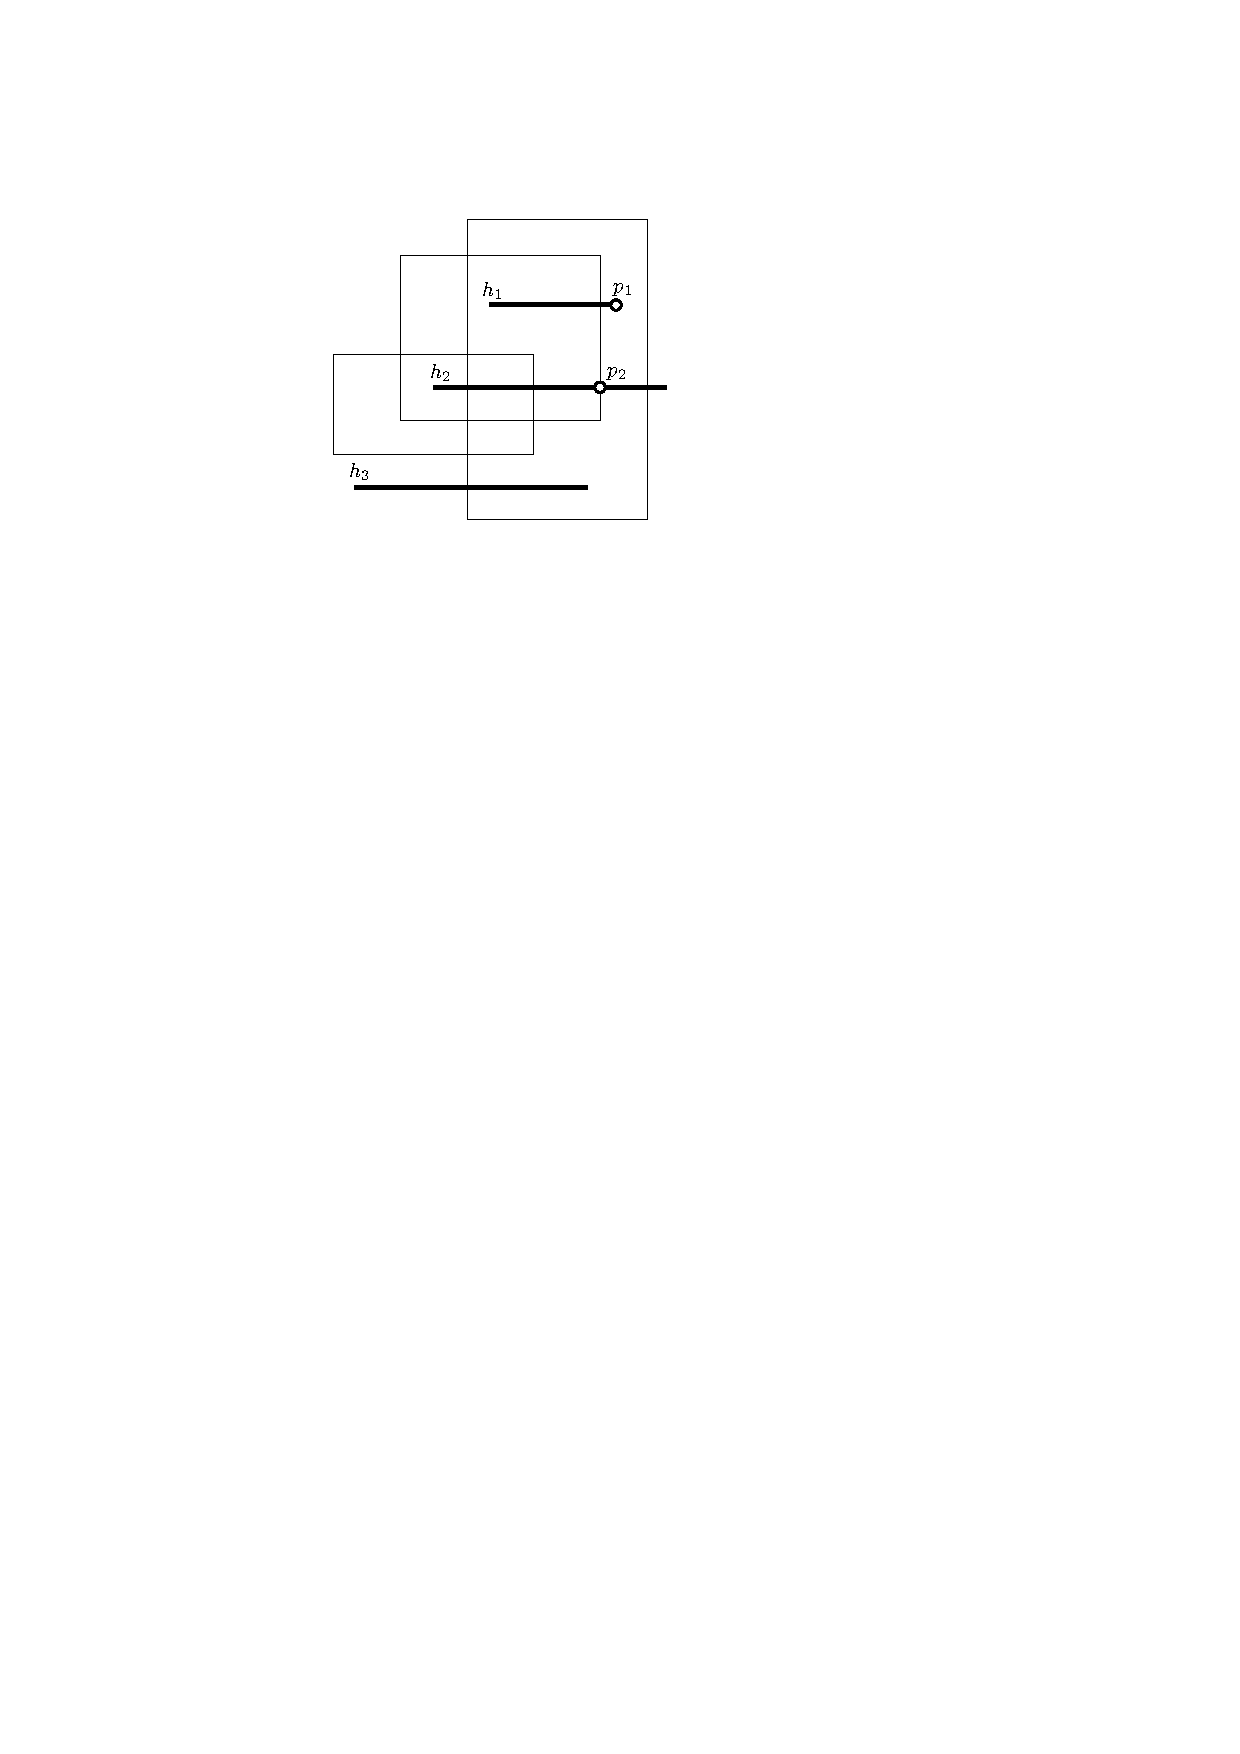
\includegraphics[height=30mm]{./artwork/prob-a} & 
        \hspace{3mm}
        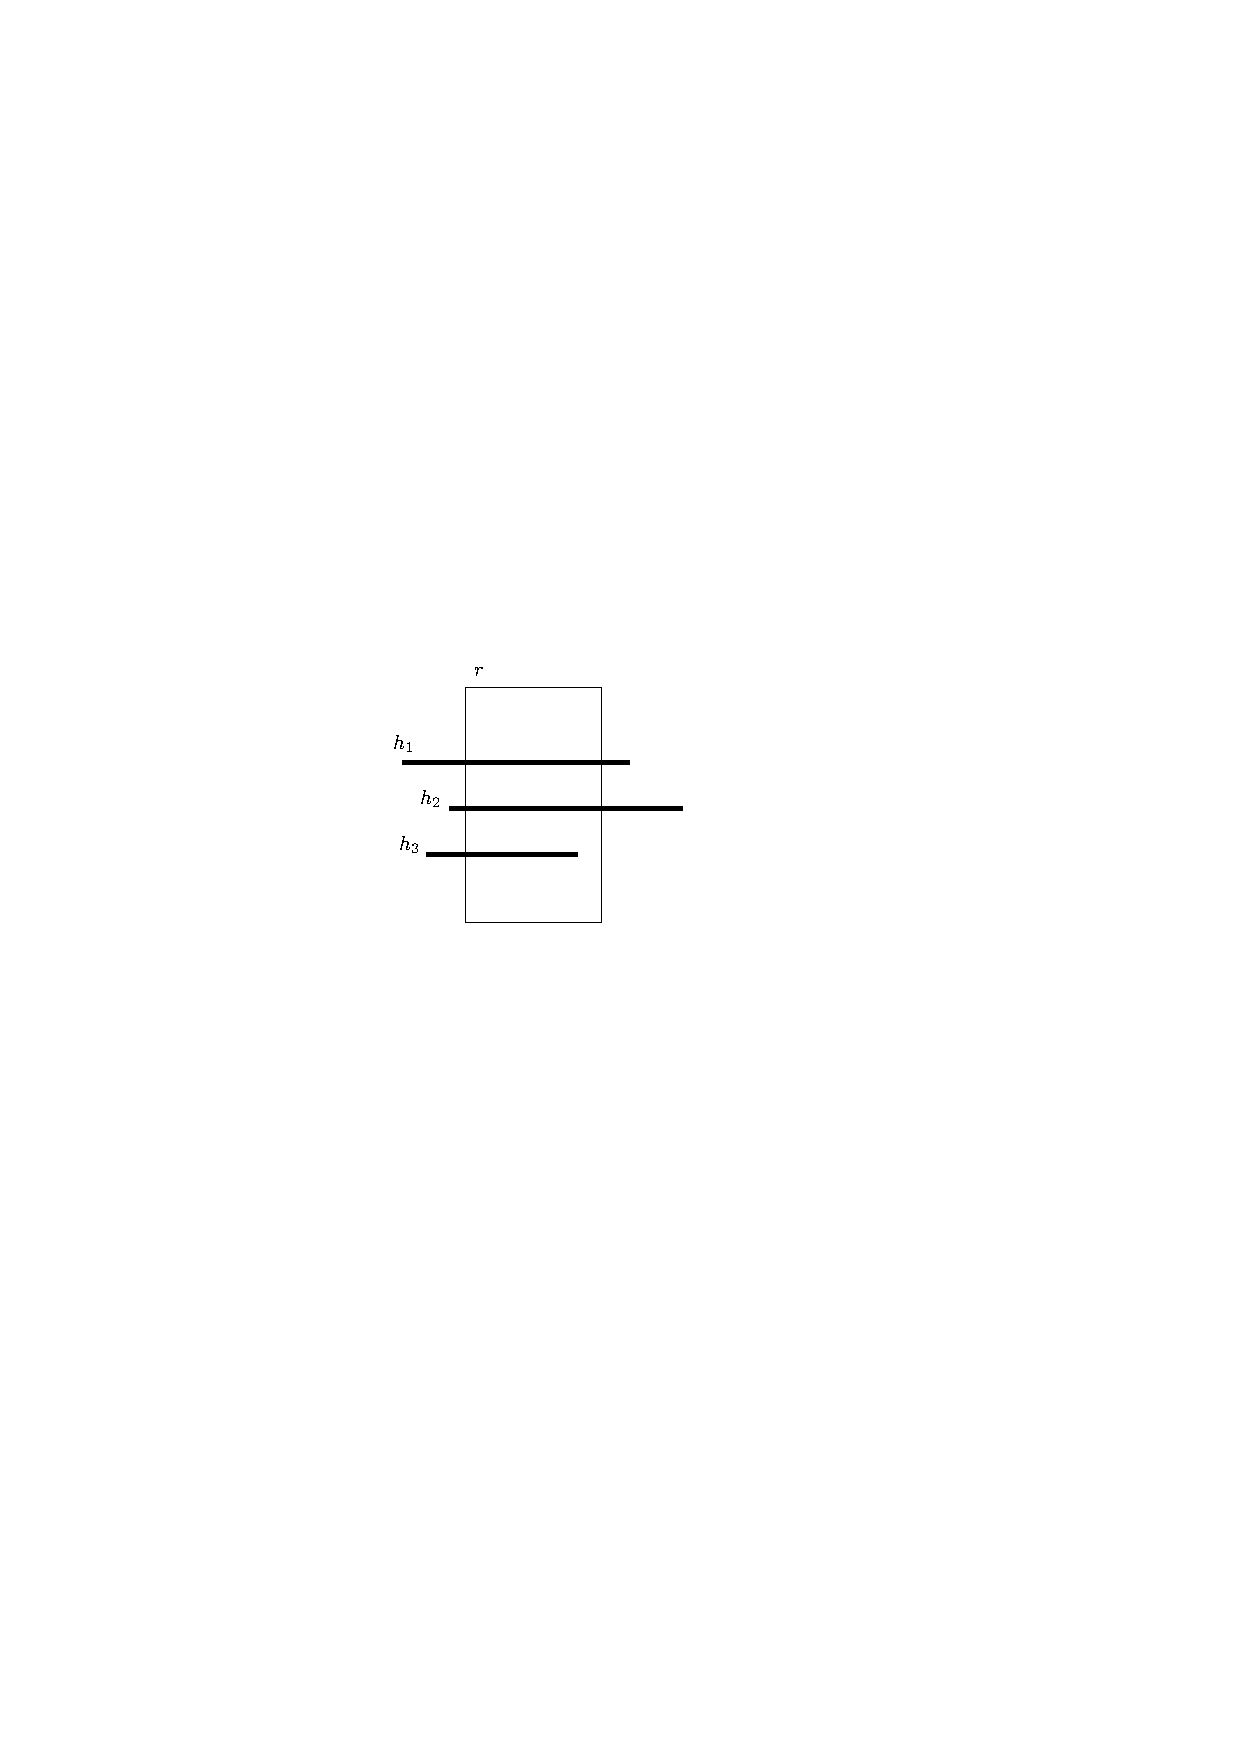
\includegraphics[height=30mm]{./artwork/prob-b} &
        \hspace{3mm}
        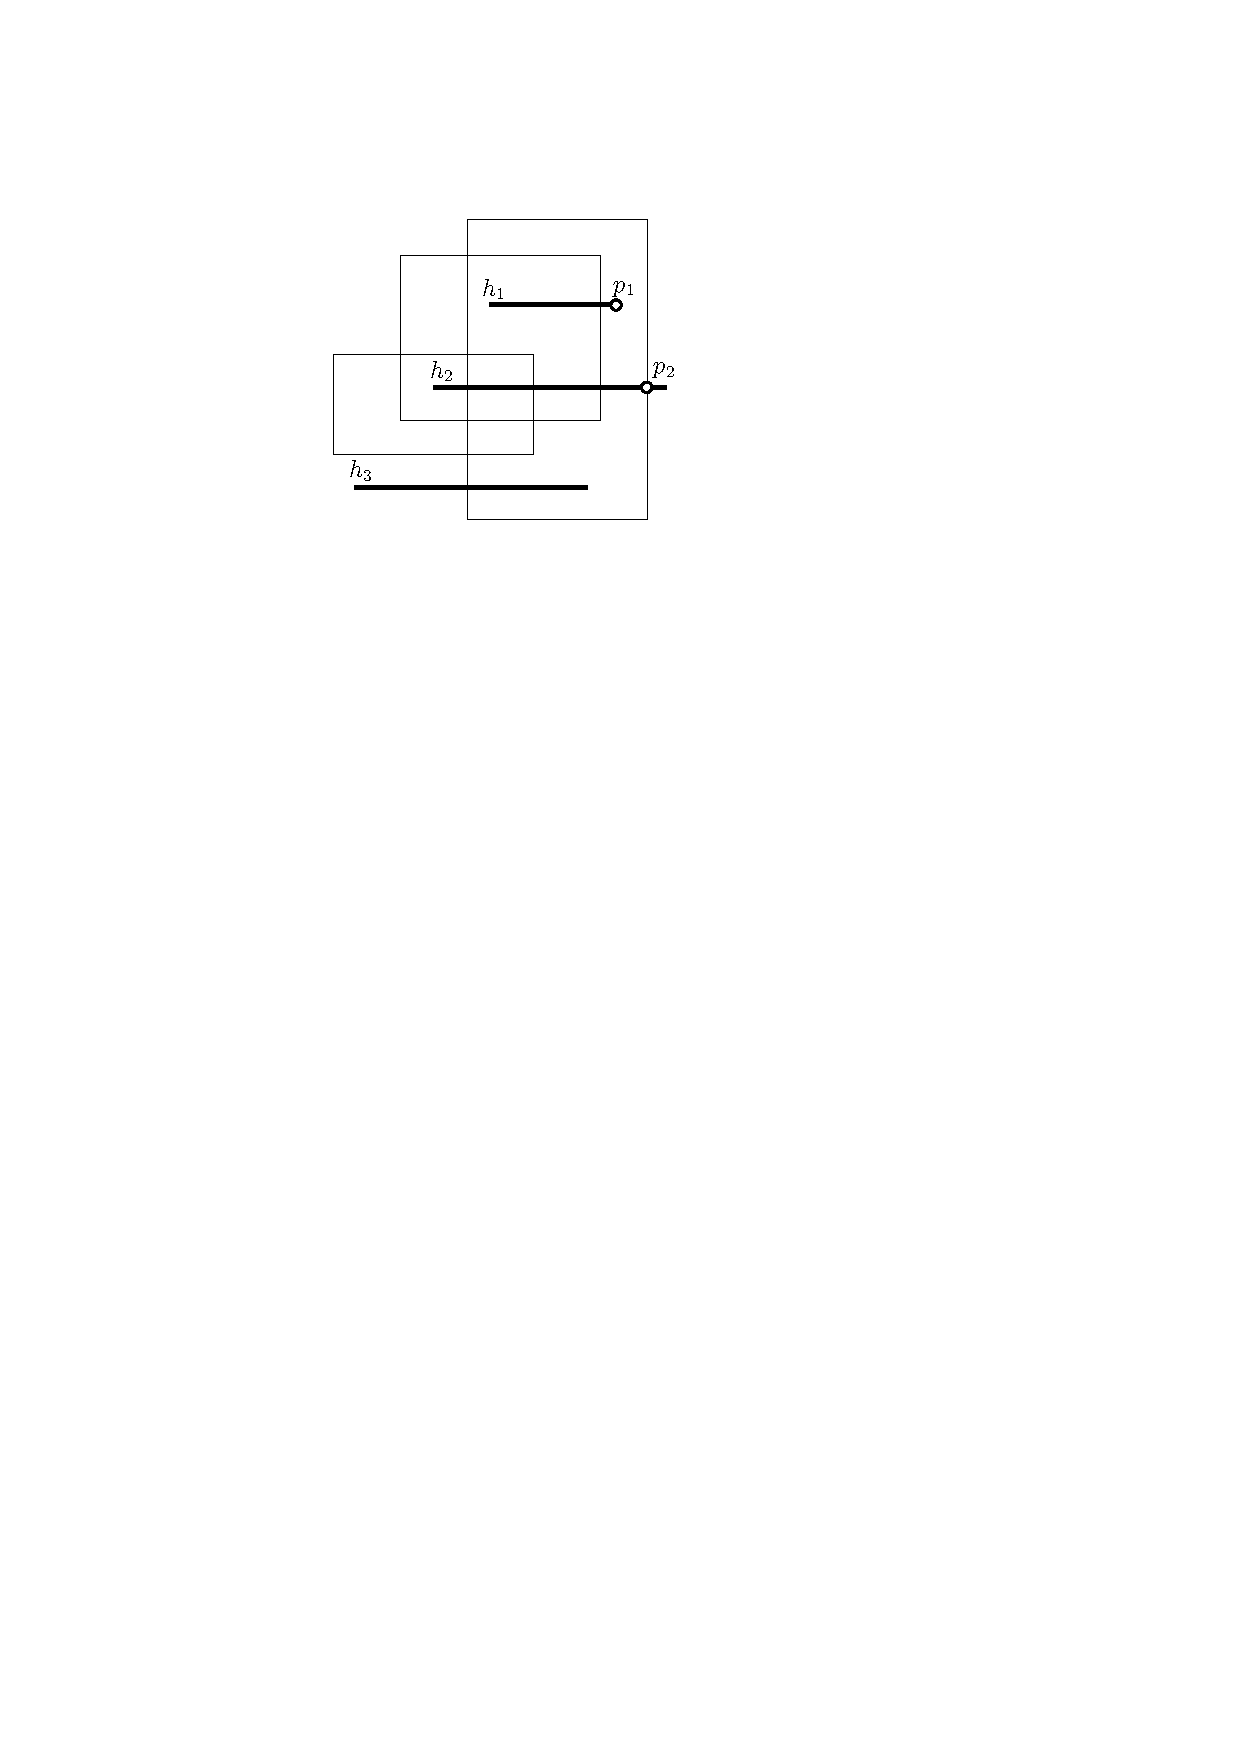
\includegraphics[height=30mm]{./artwork/prob-c} &
        \hspace{3mm}
        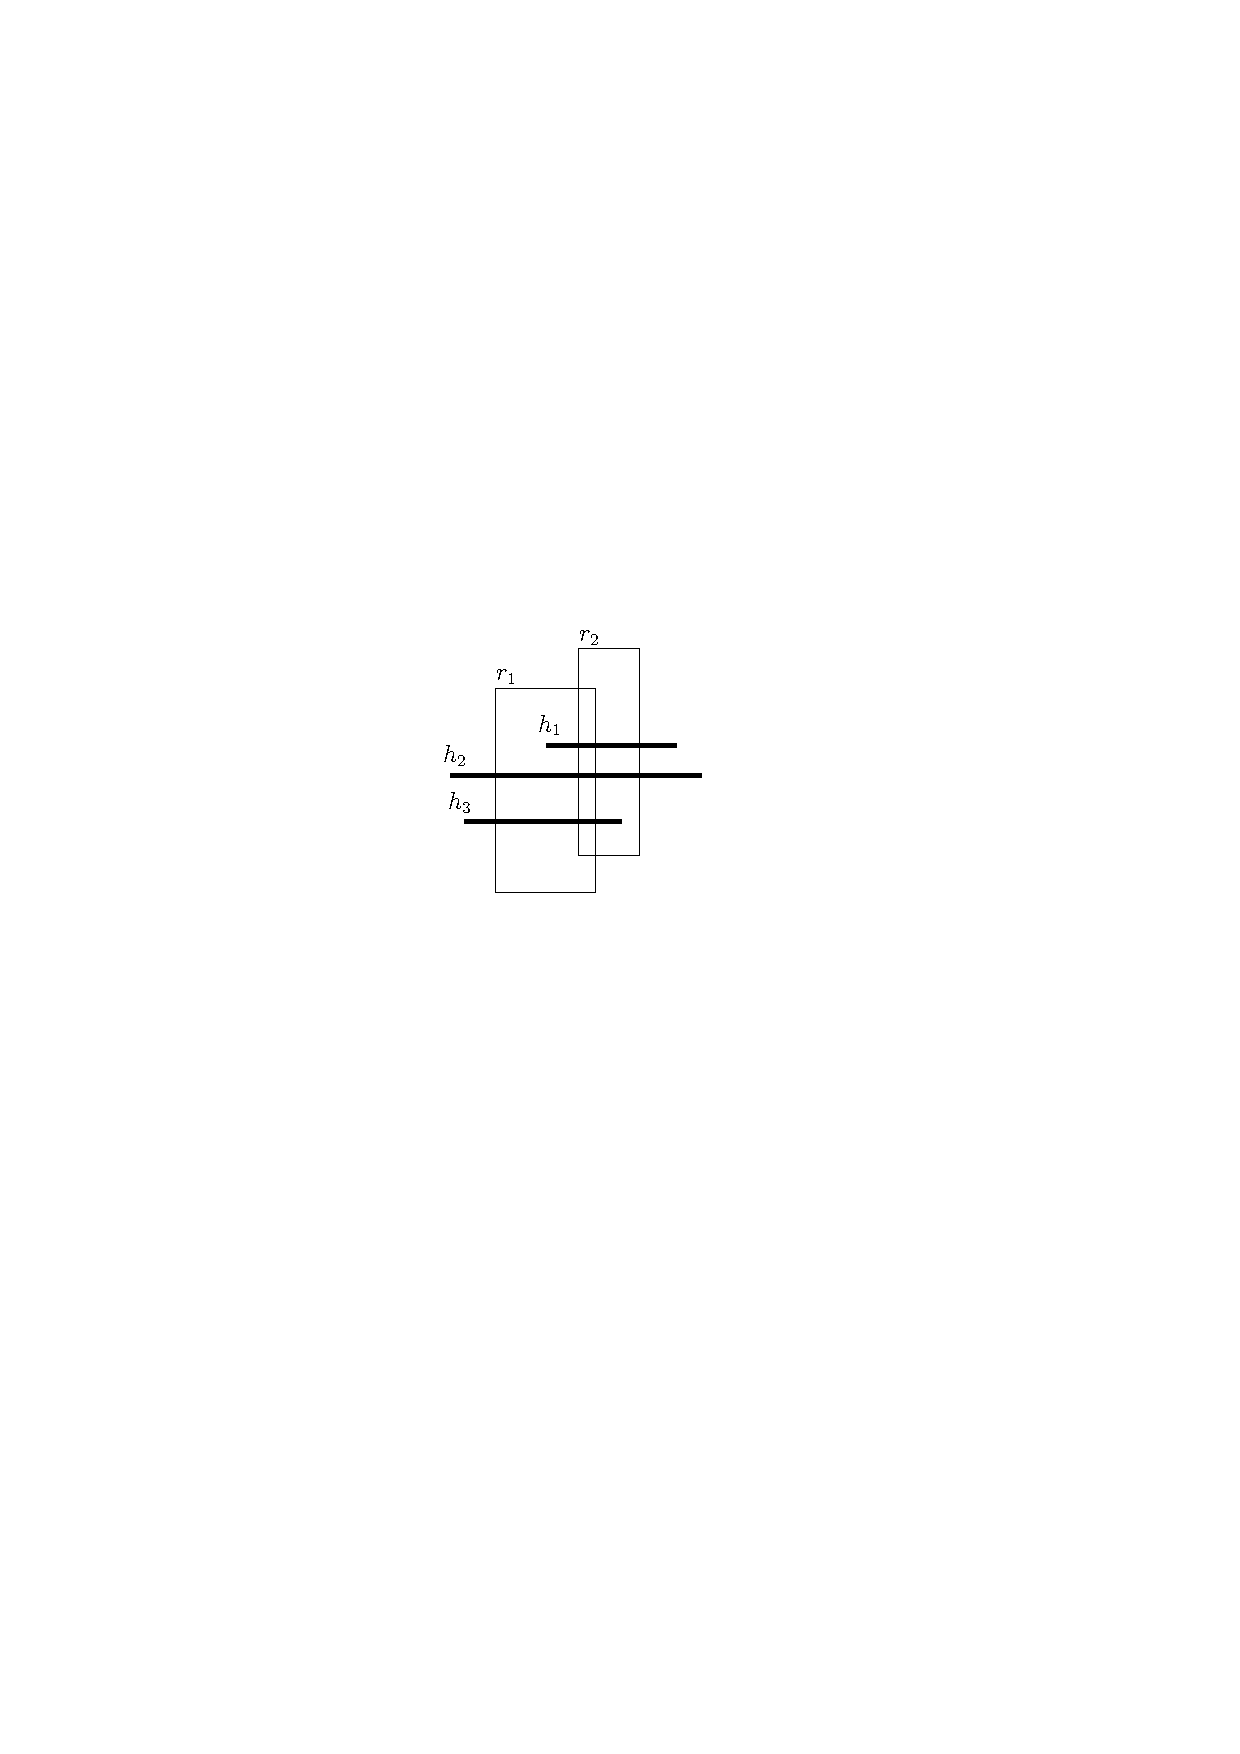
\includegraphics[height=30mm]{./artwork/prob-d} \\
        (a) Problem $\EuScript{A}$ &
        \hspace{3mm}
        (b) Problem $\EuScript{B}$ &
        \hspace{3mm}
        (c) Problem $\EuScript{C}$ &
        \hspace{3mm}
        (d) Problem $\EuScript{D}$
    \end{tabular}

    \figcapup
    \caption{Four geometric building brick problems}
    \label{fig:probs}
    \figcapdown
\end{figure*}


\extraspacing {\bf Problem $\bm{\EuScript{A}}$.} The input involves a set $H$ of horizontal segments and a set $R$ of rectangles, all in 2D space. The goal is to report, for each segment $h \in H$, the rightmost point $p$ on $h$ satisfying the condition that $p$ is covered by at least one left-end covering rectangle of $h$ in $R$ --- formally, for $h = [x_1, x_2] \times y$, we aim to find the maximum $x \in [x_1, x_2]$ such that there exists at least one rectangle $r \in R$ covering both the left end point of $h$ and the point $(x, y)$. If the point $p$ exists (equivalently, $h$ has at least one left-end covering rectangle in $R$), then we should output a tuple $(h, p)$; otherwise, we output nothing for $h$. Figure~\ref{fig:probs}a gives an example where $H = \set{h_1, h_2}$ and $R$ includes the three rectangles shown; the output is $\set{(h_1, p_1), (h_2, p_2)}$.

\vgap

In Appendix~\ref{app:prob-a}, we explain how to solve the problem in $O(n \log n)$ time where $n = |H| + |R|$.

\extraspacing {\bf Problem $\bm{\EuScript{B}}$.} The input involves a set $H$ of horizontal segments and a set $R$ of rectangles, all in 2D space. The goal is to report, for each rectangle $r \in R$, its lowest crossing segment $h \in H$ --- formally, $h = [x_1, x_2] \times y$ has the smallest $y$ coordinate among all the segments in $H$ crossing $r$. If such an $h$ does not exist, output nothing for $r$.  Figure~\ref{fig:probs}b gives an example where $H = \set{h_1, h_2, h_3}$ and $R = \set{r_1, r_2}$; the output is $\set{(r_1, h_3), (r_2, h_2)}$.

\vgap

In Appendix~\ref{app:prob-b}, we explain how to solve the problem in $O(n \log n)$ time where $n = |H| + |R|$.

\extraspacing {\bf Problem $\bm{\EuScript{C}}$.} The input involves a set $H$ of horizontal segments and a set $R$ of rectangles, all in 2D space. The goal is to report, for each segment $h \in H$, all the rectangles $r \in R$ containing $h$. Furthermore, those rectangles need to be sorted by the x-coordinates of their right boundaries. Formally, if $r_1, r_2, ..., r_t$ (for some $t \ge 1$) are all the rectangles in $R$ containing $h$, we output $(h: r_1, r_2, ..., r_t)$, provided that $x_i > x_{i-1}$ for each $i \in [2, t]$ where $x_i$ (resp., $x_{i-1}$) is the x-coordinate of the right boundary of $r_i$ (resp., $r_{i-1}$). Figure~\ref{fig:probs}c gives an example where $H = \set{h_1, h_2, h_3}$ and $R = \set{r_1, r_2, r_3}$; the output is $\set{(h_1: r_2, r_1), (h_2: r_2, r_3)}$.

\vgap

In Appendix~\ref{app:prob-c}, we explain how to solve the problem in $O(n \log n + \out)$ time where $n = |H| + |R|$ and $\out$ is the number of pairs $(h, r) \in H \times R$ such that $r$ contains $h$.

\extraspacing {\bf Problem $\bm{\EuScript{D}}$.} The input involves a set $H$ of horizontal segments and a set $R$ of rectangles, all in 2D space. The goal is to report, for each rectangle $r \in R$, all the segments $h \in H$ crossing $r$. Furthermore, those segments need to be sorted by their y-coordinates. Formally, if $h_1, h_2, ..., h_t$ (for some $t \ge 1$) are all the segments in $H$ crossing $r$, we output $(r: h_1, h_2, ..., h_t)$, provided that $y_i > y_{i-1}$ for each $i \in [2, t]$ where $y_i$ (resp., $y_{i-1}$) is the y-projection of $h_i$ (resp., $h_{i-1}$). Figure~\ref{fig:probs}d gives an example where $H = \set{h_1, h_2, h_3}$ and $R = \set{r_1, r_2}$; the output is $\set{(r_1: h_3, h_2), (r_2: h_2, h_1)}$.

\vgap

In Appendix~\ref{app:prob-d}, we explain how to solve the problem in $O(n \log n + \out)$ time where $n = |H| + |R|$ and $\out$ is the number of pairs $(h, r) \in H \times R$ such that $h$ crosses $r$.

\section{H-V Multiway Spatial Joins} \label{sec:hv}

This section deals with a special version of the $k$-SJ problem. Recall that the input of $k$-SJ comprises $k$ sets of rectangles: $R_1, R_2, ..., R_k$. In the special version --- which we name the {\em H-V $k$-SJ} problem ---  we impose the constraints that (i) $k \ge 3$, (ii) $R_{k-1}$ should be a set of horizontal segments, and (iii) $R_k$ should be a set of vertical segments. For better clarity, we will represent the input sets as $R_1, R_2, ..., R_{k-2}, H$ ($=R_{k-1}$), and $V$ ($=R_k$). Remember that each $R_i$ ($i \in [k-2]$) is a set of rectangles. As shown in the next section, solving the H-V $k$-SJ problem is an imperative step for settling the original $k$-SJ problem. 

\vgap 

Our objective is to prove that the H-V $k$-SJ problem can be reduced to the $(k-1)$-SJ problem --- note: it is $(k-1)$-SJ here, rather than H-V $(k-1)$-SJ. For this purpose, we assume the existence of an algorithm $\A$ that can solve $\kappa$-SJ problems for all $\kappa \in [2, k-1]$. Denote by 
\myitems{
    \item $F_\kappa(n, \out)$ the worst-case runtime of $\A$ on any instance of $\kappa$-SJ that has input size $n$ and output size $\out$;
    \item $G_\kappa(n, \out)$ the worst-case space consumed by $\A$ on any instance mentioned above.
}
We consider that $F_\kappa(n, \out) \le F_{\kappa + 1}(n, \out)$ and $G_\kappa(n, \out) \le G_{\kappa + 1}(n, \out)$ for any $\kappa \in [2, k-2]$, that is, its overhead on $\kappa$-SJ should not be larger than that on $(\kappa+1)$-SJ.

\vgap

The rest of the section serves as a proof for: 

\begin{lemma} \label{lmm:hv}
    The H-V $k$-SJ problem can be solved in 
    \myeqn{
        O(k) \cdot \big( F_{k-1}(n, \out) + n\log n + \out \big) \nn 
    }
    time using $O(n + \out) + G_{k-1}(n, \out)$ space.
\end{lemma}

\subsection{Categorizing the Result Tuples} \label{sec:hv:result-part}

Let us represent the result of the H-V $k$-SJ problem as $\J_k(R_1, ..., R_{k-2},$ $H, V)$. Recall that $\J_k(R_1, ..., R_{k-2},$ $H, V)$ contains all such $k$-tuples $(r_1, ..., r_{k-2}, h, v) \in R_1 \times ... \times R_{k-2} \times H \times V$ satisfying the condition that $h \cap v \bigcap_{i=1}^{k-2} r_i$ is not empty. The condition is equivalent to saying that the intersection point of $h$ and $v$ falls in every $r_i$ of $i \in [k-2]$.

\vgap

Let us focus on any $k$-tuple $(r_1, ..., r_{k-2}, h, v) \in  \J_k(R_1, ..., R_{k-2},$ $H, V)$. We classify the tuple into one of the two categories below: 

\myitems{
    \item {{\bf Type 1:}} $h$ crosses all of $r_1, ..., r_{k-2}$, and $v$  crosses all of $r_1, ..., r_{k-2}$; 
    
    \item {{\bf Type 2:}} $h$ or $v$ fails to cross some rectangle in $\set{r_1, r_2, ..., r_{k-2}}$. This means the existence of at least one rectangle $r_i$ (for some $i \in [k-2]$) that covers an endpoint of either $h$ or $v$ or both.
}
Figure~\ref{fig:hv:types} illustrates a result tuple of each type, assuming $k = 4$.

\begin{figure} 
    \begin{tabular}{cc} 
        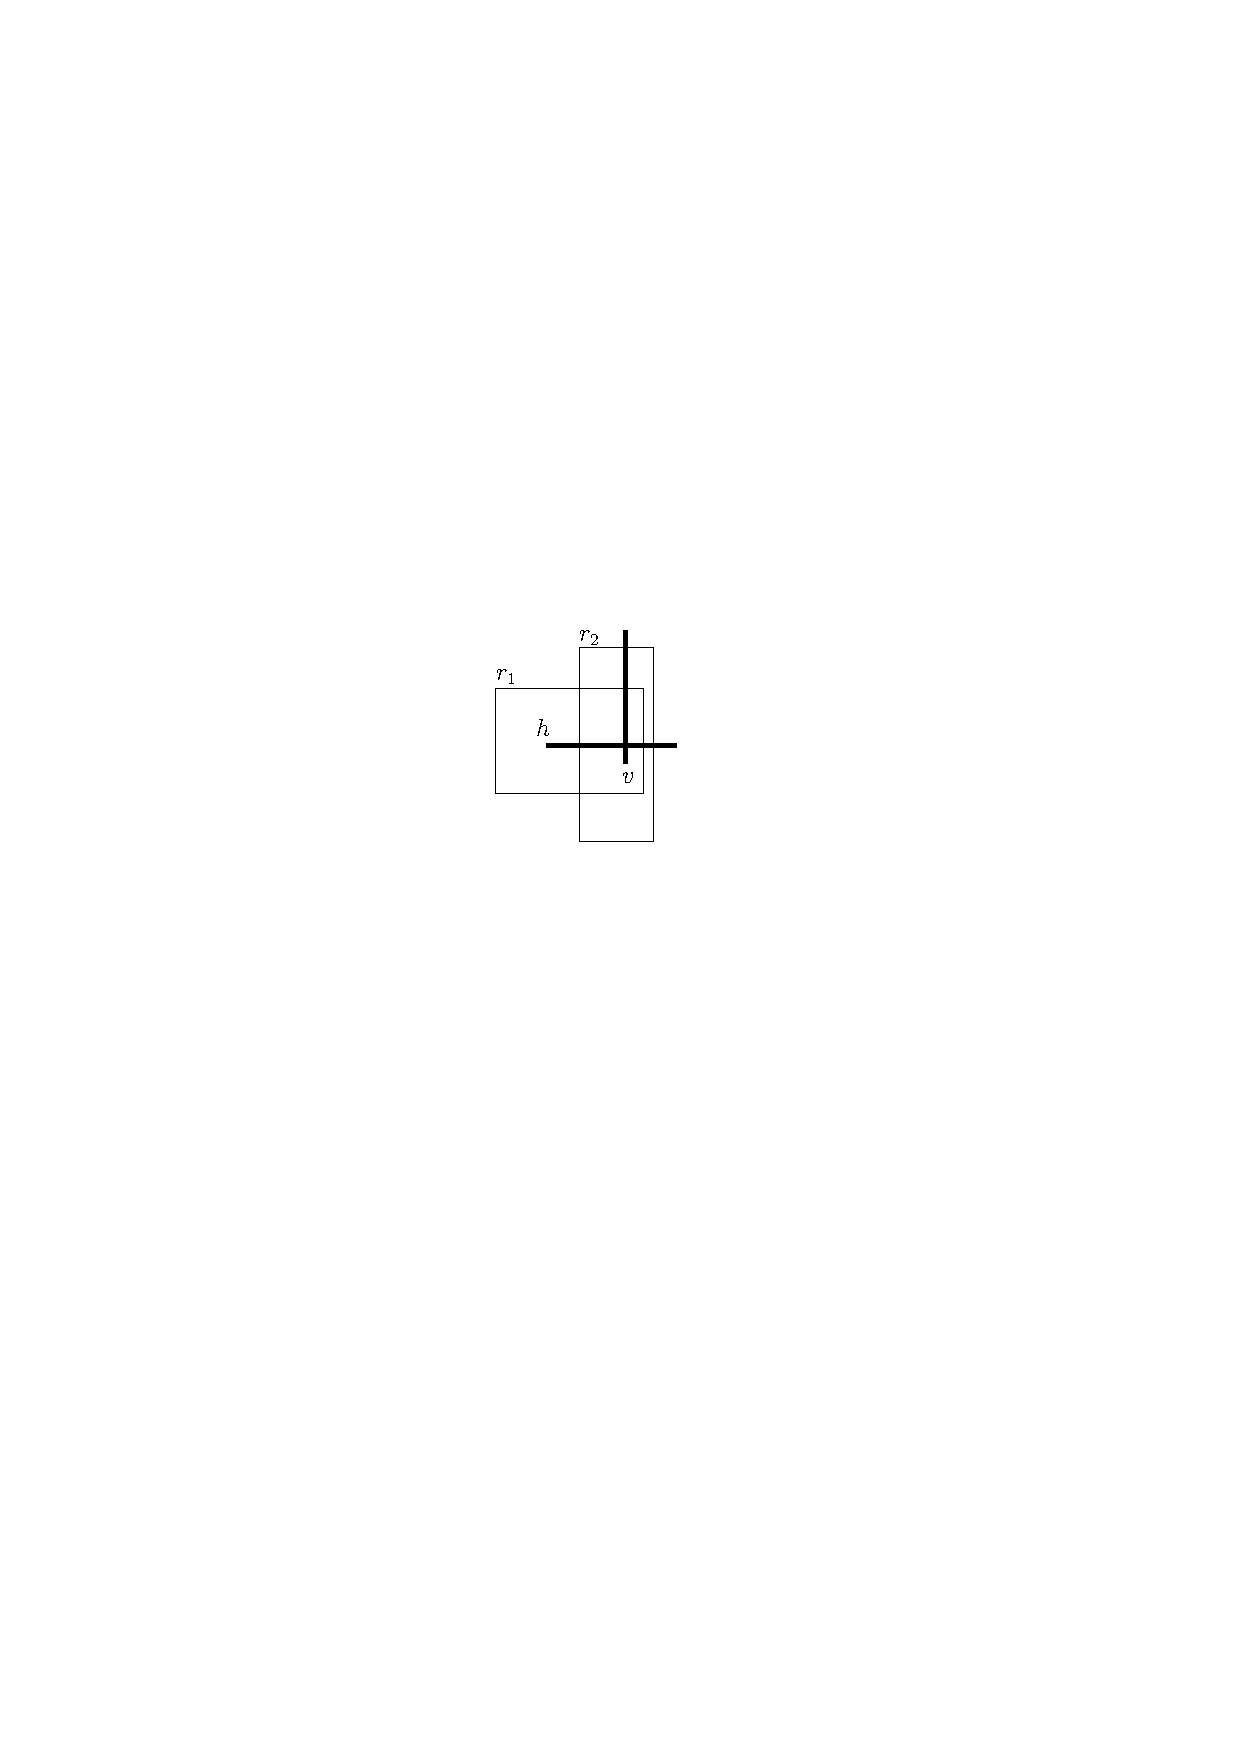
\includegraphics[height=27mm]{./artwork/type1} & 
        \hspace{5mm} 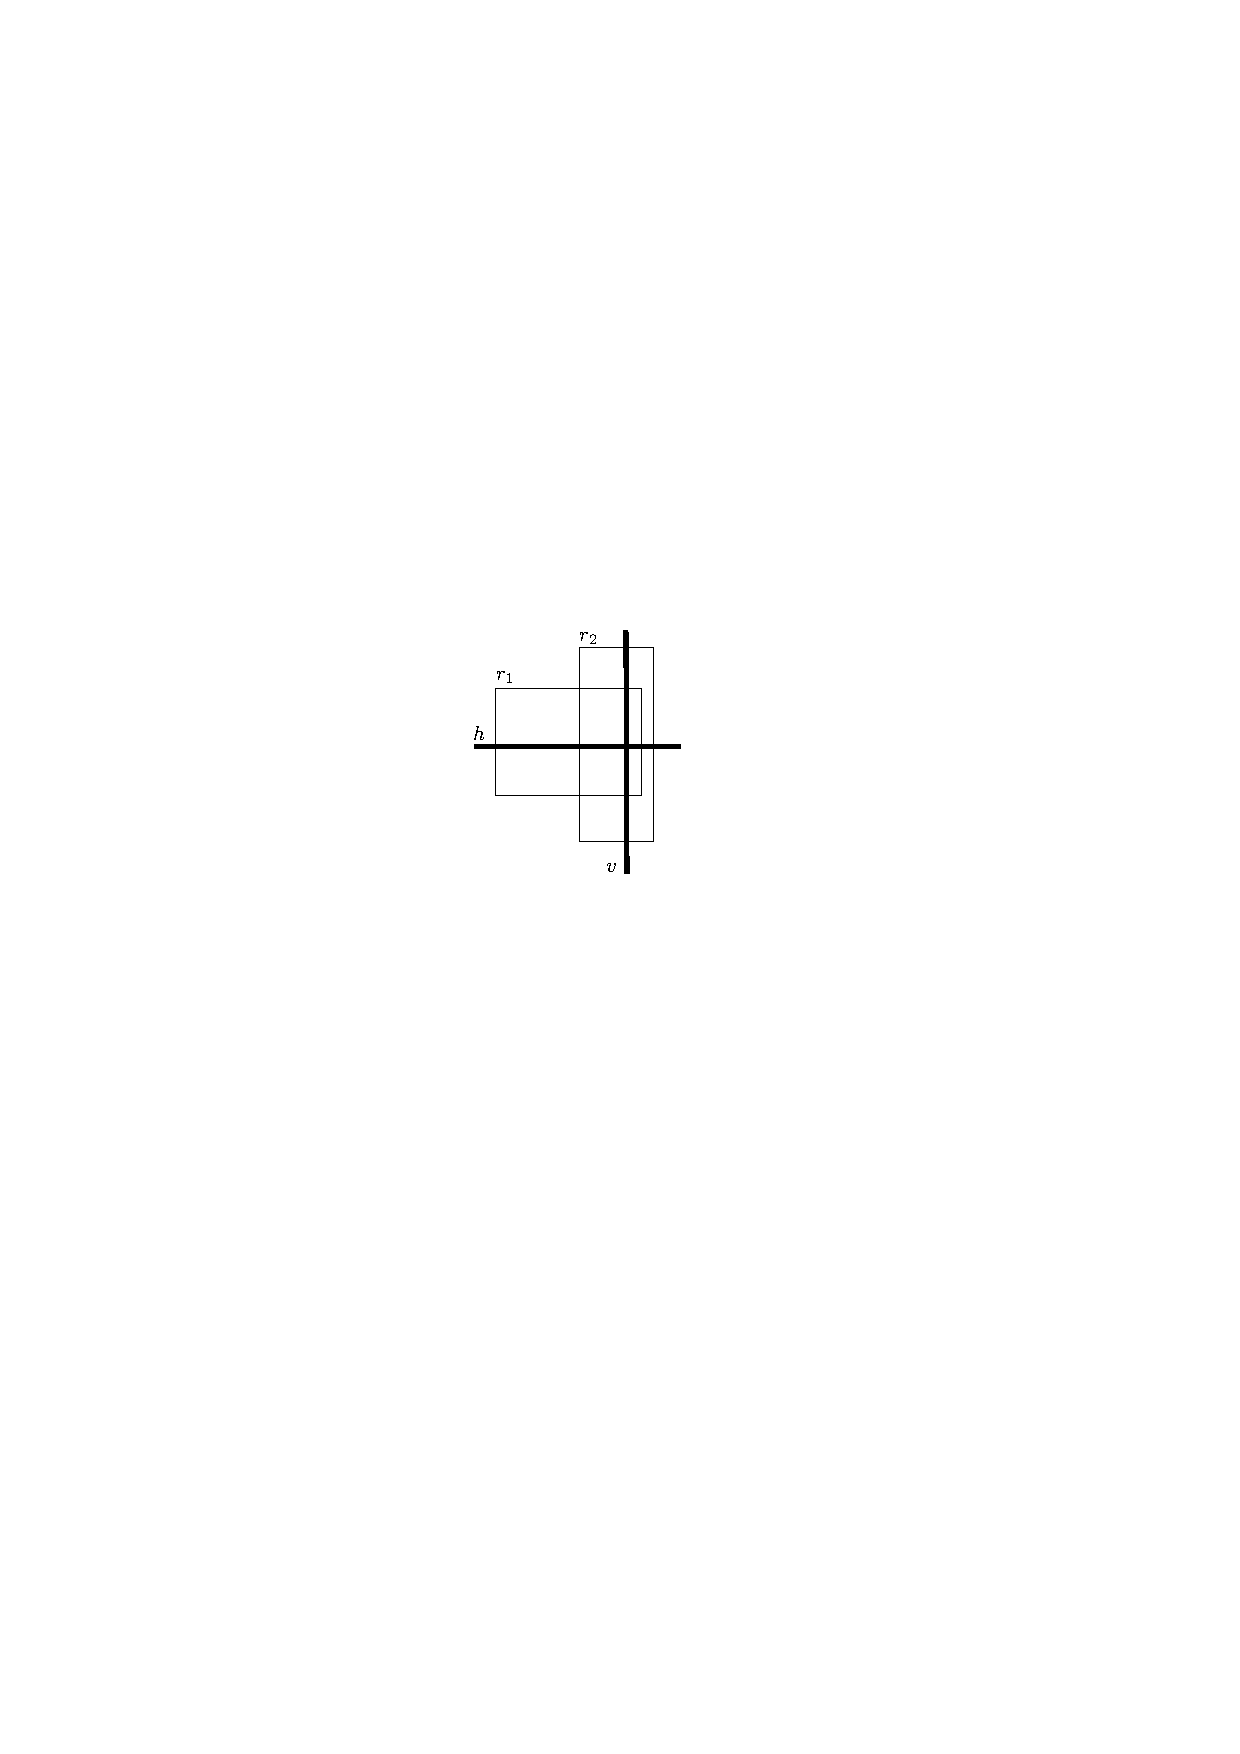
\includegraphics[height=27mm]{./artwork/type2} \\
        (a) Cat.\ 1 result tuple & 
        (b) Cat.\ 2 result tuple
    \end{tabular}
    
    \figcapup 
    \caption{Two categories of H-V $k$-SJ result tuples ($k$ = 4)} 
    \label{fig:hv:types}
    \figcapdown
\end{figure}

\vgap 

We will find result tuples of each type separately. Before proceeding, however, let us observe a sense of symmetry for Type 2. As mentioned, for a result tuple $(r_1, ..., r_{k-2}, h, v)$ of this type, a rectangle $r_i$, for some $i \in [k-2]$, covers an endpoint of $h$ or $v$ or both. As (i) there are $k-2$ choices for $i$ and (ii) $h$ and $v$ together have four endpoints, we can divide Type 2 further into $4(k-2)$ ``sub-types'': e.g., in subtype 1 (resp., 2), $r_1$ covers the left (resp., right) endpoint of $h$, in subtype 3 (resp., 4), $r_1$ covers the bottom (resp., top) endpoint of $v$, in subtype 5 (resp., 6), $r_2$ covers the left (resp., right) endpoint of $h$, etc. It is possible for the result tuple to belong to multiple sub-types simultaneously.

\vgap 

Our subsequent discussion will proceed as follows.  Section~\ref{sec:hv:type1} will explain how to produce all the result tuples of Type 1. Section~\ref{sec:hv:type2} will explain how to produce the result tuples $(r_1, ..., r_{k-2}, h, v)$ of a particular sub-type of Type 2: those tuples where $r_1$ covers the left endpoint of $h$. Other sub-types can be computed using the same algorithm, by symmetry.

\vgap 

A remark is in order about duplicate removal. A result tuple of Type 2 can belong to, in the worst case, all the $4(k-2)$ sub-types. Hence, by considering each sub-type separately, we may see the same result tuple multiple times (precisely, up to $4(k-2)$ times) in the whole algorithm. However, this does {\em not} mean that the tuple need to be {\em reported} multiple times. Whenever a Type-2 result tuple is found, we can immediately decide all the sub-types it belongs to. To avoid outputting the tuple more than once, we can enforce a policy to designate a specific sub-type for outputting. One such policy is the following: among all sub-types that the tuple belongs to, identify the one with the smallest sub-type number $t$ (an integer from 1 to $4(k-2)$); report the tuple only when we are computing the particular sub-type $t$.

\subsection{Finding Result Tuples of Type 1} \label{sec:hv:type1}

\subsection{Finding Result Tuples of Type 2} \label{sec:hv:type2}

\todo{Remark on Rahul's result}

\bibliographystyle{plainurl}% the mandatory bibstyle
\bibliography{ref}

\balance

\appendix 

\section{Algorithm for Problem $\bm{\EuScript{A}}$} \label{app:prob-a}

\section{Algorithm for Problem $\bm{\EuScript{B}}$} \label{app:prob-b}

\section{Algorithm for Problem $\bm{\EuScript{C}}$} \label{app:prob-c}

\section{Algorithm for Problem $\bm{\EuScript{D}}$} \label{app:prob-d}

\section{An $\bm{\Omega(n \log n)}$ Lower Bound for 2-SJ} \label{app:lb}

\section{Hardness of 3-SJ in 3D Space} \label{app:lb-cond}

%\end{sloppy}
\end{document}

